
\subsection{Electrodes}

\begin{frame}
  \frametitle{Input options}
  \framesubtitle{Electrodes}

  \begin{itemize}
    \item Electrodes are defined individually, all settings are on a \emph{per electrode} basis
    \item Beware of indices of electrodes in the device region
    \item Beware of semi-infinite directions (the semi-infinite direction points
    \emph{away} from the device region)

  \end{itemize}
  
\end{frame}

\begin{frame}[label=electrode]
  \frametitle{Input options}
  \framesubtitle{Electrodes}

  \only<1>{Define names of electrodes}%
  \only<2>{Define each electrode}%
  \only<3>{Assert that the electrode settings reflect the input\footnote{\emph{HINT}: Do \emph{NOT} specify
          \texttt{used-atoms} if you use \emph{ALL} atoms!}}%
  \only<4>{When reducing the used atoms, it becomes slightly more difficult}%
  \only<5>{Automatically detects semi-infinite lattice vectors}%
  \only<6>{Buffer atoms removed from TBtrans/TranSiesta SCF cycle}%

  \begin{tikzpicture}[thick,left/.style={densely dotted,color=bad},
    right/.style={color=ok}]

    % Define the electrode and we are done
    \begin{scope}
      \matrix {
          \node[fdf] {\%block TS.Elecs}; \\
          \node[fdf,ind,lmark] (left) {Left}; \\
          \node[fdf,ind,lmark] (right) {Right}; \\
          \node[fdf,ind] {...}; \\
          \node[fdf] {\%endblock}; \\
      };
    \end{scope}
    
    \uncover<2->{
        \begin{scope}[xshift=4.5cm,yshift=1.5cm]
          \matrix {
              \node[fdf,rmark] (l) {\%block TS.Elec.Left}; \\
              \node[fdf,ind] (l-HS) {HS <TSHS-file>/<nc-file>}; \\
              \node[fdf,ind] {chem-pot <in TS.ChemPots>}; \\
              \alt<3>{
                  \node[fdf,ind,left] (l-pos) {elec-pos 1}; \\
              }{
                  \node[fdf,ind] (l-pos) {elec-pos 1}; \\
              }
              \alt<4-5>{
                  \node[fdf,ind,left] (l-semi) {semi-inf-dir -a2}; \\
              }{
                  \node[fdf,ind] (l-semi) {semi-inf-dir -a2}; \\
              }
              \alt<4,6>{
                  \node[fdf,ind,left] (l-used) {used-atoms 3}; \\
              }{
                  \node[fdf,ind] (l-used) {used-atoms 4}; \\
              }
              \node[fdf,ind] (l-bloch) {bloch 1 1 1}; \\
              \node[fdf,ind] (l-eta) {eta <energy>}; \\
              \node[fdf] {\%endblock};\\
          };
        \end{scope}
        \draw[->] (left) -- ++(1.5,0) to[out=0,in=180] (l);

        \begin{scope}[xshift=4.5cm,yshift=-3.5cm]
          \matrix {
              \node[fdf,rmark] (r) {\%block TS.Elec.Right}; \\
              \node[fdf,ind] (r-HS) {HS <TSHS-file>/<nc-file>}; \\
              \node[fdf,ind] {chem-pot <in TS.ChemPots>}; \\
              \alt<3>{
                  \node[fdf,ind,right] (r-pos) {elec-pos end -1}; \\
              }{
                  \node[fdf,ind] (r-pos) {elec-pos end -1}; \\
              }
              \alt<4-5>{
                  \node[fdf,ind,right] (r-semi) {semi-inf-dir +a2}; \\
              }{
                  \node[fdf,ind] (r-semi) {semi-inf-dir +a2}; \\
              }
              \alt<4>{
                  \node[fdf,ind,right] (r-used) {used-atoms 3}; \\
              }{
                  \node[fdf,ind] (r-used) {used-atoms 4}; \\
              }
              \node[fdf,ind] {...}; \\
              \node[fdf] {\%endblock};\\
          };
        \end{scope}

        \draw[->] (right) -- ++(1,0) to[out=0,in=180] (r);
        
    }

    \uncover<3->{
        \begin{scope}[xshift=12.75cm,yshift=3cm]
          \begin{scope}[scale=0.7,
            every node/.style={scale=0.7,
                inner sep=.01ex,outer sep=.01ex,
            }]
            \matrix {
                \node[fdf] {\%block Atomic...Species}; \\
                \node[fdf,ind] (1) {\texttt{0. 0. 0.0  1}}; \\
                \node[fdf,ind] (2) {\texttt{0. 0. 1.5  1}}; \\
                \node[fdf,ind] (3) {\texttt{0. 0. 3.0  1}}; \\
                \node[fdf,ind] (4) {\texttt{0. 0. 4.5  1}}; \\
                \node[fdf] {\%endblock};\\
                \node[fdf] {\%block LatticeVectors}; \\
                \node[fdf,ind] {\texttt{ 0. 10.  0.}}; \\
                \alt<5>{
                    \node[fdf,ind,rmark] (e-A2) {\texttt{ 0.  0.  6.}}; \\
                }{
                    \node[fdf,ind] (e-A2) {\texttt{ 0.  0.  6.}}; \\
                }
                \node[fdf,ind] {\texttt{10.  0.  0.}}; \\
                \node[fdf] {\%endblock};\\
            };
          \end{scope}


          \begin{scope}[yshift=-5cm,scale=0.7,
            every node/.style={scale=0.7,
                inner sep=.01ex,outer sep=.01ex,
            }]
            \matrix {
                \node[fdf] {\%block Atomic...Species}; \\
                \alt<6>{
                    \node[fdf,ind,gray,rmark] (L1) {\texttt{0. 0.  0.0  1}}; \\
                }{
                    \node[fdf,ind] (L1) {\texttt{0. 0.  0.0  1}}; \\
                }
                \node[fdf,ind] (L2) {\texttt{0. 0.  1.5  1}}; \\
                \node[fdf,ind] (L3) {\texttt{0. 0.  3.0  1}}; \\
                \node[fdf,ind] (L4) {\texttt{0. 0.  4.5  1}}; \\
                \node[fdf,ind] {\texttt{0. 0.  6.0  1}}; \\
                \node[fdf,ind] {\texttt{0. 0.  7.5  1}}; \\
                \node[fdf,ind] {\texttt{0. 0.  9.0  1}}; \\
                \node[fdf,ind] {\texttt{0. 0. 10.5  1}}; \\
                \node[fdf,ind] {\texttt{0. 0. 12.0  1}}; \\
                \node[fdf,ind] {\texttt{0. 0. 13.5  1}}; \\
                \node[fdf,ind] (R4) {\texttt{0. 0. 15.0  1}}; \\
                \node[fdf,ind] (R3) {\texttt{0. 0. 16.5  1}}; \\
                \node[fdf,ind] (R2) {\texttt{0. 0. 18.0  1}}; \\
                \node[fdf,ind] (R1) {\texttt{0. 0. 19.5  1}}; \\
                \node[fdf] {\%endblock};\\
                \node[fdf] {\%block LatticeVectors}; \\
                \alt<5>{
                    \node[fdf,ind,rmark] (d-A1) {\texttt{ 0.  0. 21.}}; \\
                }{
                    \node[fdf,ind] (d-A1) {\texttt{ 0.  0. 21.}}; \\
                }
                \node[fdf,ind] {\texttt{ 0. 10.  0.}}; \\
                \node[fdf,ind] {\texttt{10.  0.  0.}}; \\
                \node[fdf] {\%endblock};\\
            };
          \end{scope}
        \end{scope}
  }


  \only<3>{
      \draw[decorate, decoration=brace]
      ($(4.south west)+(-0.1,0)$) -- ($(1.north west)+(-0.1,0)$) coordinate[midway] (full elec);
      \draw[->, s >] (l-used) to[out=0,in=180] (full elec);
      \draw[->, s >] (r-used) to[out=0,in=180] (full elec);

      \draw[->, s >,left] (l-pos) to[out=0,in=180] (L1);
      \draw[->, s >,right] (r-pos) to[out=0,in=180] (R1);

  }

  \only<4>{
      \draw[decorate, decoration=brace,left]
      ($(4.south west)+(-0.1,0)$) -- ($(2.north west)+(-0.1,0)$) coordinate[midway] (left elec);
      \draw[decorate, decoration=brace,right]
      ($(3.south west)+(-0.6,0)$) -- ($(1.north west)+(-0.6,0)$) coordinate[midway] (right elec);

      \draw[decorate, decoration=brace,left]
      ($(L3.south west)+(-0.1,0)$) -- ($(L1.north west)+(-0.1,0)$) coordinate[midway] (left dev);
      \draw[decorate, decoration=brace,right]
      ($(R1.south west)+(-0.1,0)$) -- ($(R3.north west)+(-0.1,0)$) coordinate[midway] (right dev);

      \draw[->,s >,left] (l-used) to[out=0,in=180] (left elec);
      \draw[->,s >,right] (r-used) to[out=0,in=180] (right elec);

      \draw[<->,s <>,left] (left elec) to[out=180,in=180] (left dev);
      \draw[<->,s <>,right] (right elec) to[out=180,in=180] (right dev);

  }

  \only<5>{
      \draw[->,left,s >] (l-semi) to[out=0,in=180] (e-A2);
      \draw[->,right,s >] (r-semi.east) -- ++(0.5,0) to[out=0,in=180] (e-A2);

      \draw[<->,s <>] (d-A1) to[out=180,in=180] (e-A2);

  }

  \only<6>{
      \begin{scope}[xshift=9cm,yshift=-4.5cm]
        \matrix {
          \node[fdf] {\%block TS.Atoms.Buffer}; \\
          \node[fdf,ind,lmark] (buf) {atom 1}; \\
          \node[fdf] {\%endblock}; \\
      };
      \end{scope}
      \draw[->] (buf) to[out=0,in=180] (L1);

      \draw[decorate, decoration=brace,left]
      ($(4.south west)+(-0.1,0)$) -- ($(2.north west)+(-0.1,0)$) coordinate[midway] (left ELEC);
      \draw[decorate, decoration=brace,right]
      ($(4.south west)+(-0.6,0)$) -- ($(1.north west)+(-0.6,0)$) coordinate[midway] (right ELEC);

      \draw[decorate, decoration=brace,left]
      ($(L4.south west)+(-0.1,0)$) -- ($(L2.north west)+(-0.1,0)$) coordinate[midway] (left DEV);
      \draw[decorate, decoration=brace,right]
      ($(R1.south west)+(-0.1,0)$) -- ($(R4.north west)+(-0.1,0)$) coordinate[midway] (right DEV);

      \draw[->,s >,left] (l-used) to[out=0,in=180] (left ELEC);
      \draw[->,s >,right] (r-used) to[out=0,in=180] (right ELEC);

      \draw[<->,s <>,left] (left ELEC) to[out=180,in=180] (left DEV);
      \draw[<->,s <>,right] (right ELEC) to[out=180,in=180] (right DEV);
      
  }
      
  \end{tikzpicture}

  \only<6>{\hfill \hyperlink{algorithm<1>}{\beamergotobutton{Go to NEGF Algorithm in TBtrans}}}

\end{frame}

\begin{frame}
  \frametitle{Input options}
  \framesubtitle{Electrodes}

  \begin{center}
    Let us go through that again!
  \end{center}

\end{frame}

\againframe{electrode}

\begin{frame}
  \frametitle{Input options}
  \framesubtitle{Bloch's theorem}

  \begin{block}{Bloch's theorem}

    Extend a principle system into a bigger, but otherwise equivalent system?

    \begin{center}
      \def\mysize{6pt}
      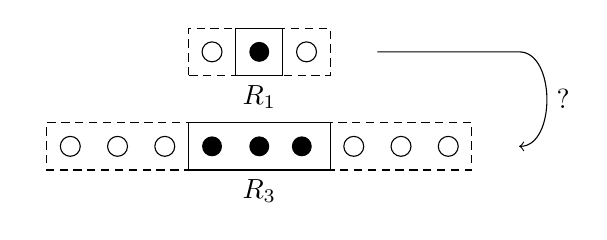
\begin{tikzpicture}[scale=.6]

        \node[left] at (-1,0) {$\hdots$};
        \draw[densely dashed] (-1,-.5) rectangle ++(1,1);
        \draw (0,-.5) rectangle ++(1,1);
        \node[below] at (.5,-.5) {$R_1$};
        \draw[densely dashed] (1,-.5) rectangle ++(1,1);
        \node[right] at (2,0) {$\hdots$};
        \coordinate (small) at (3,0);
        
        \fill (.5,0) circle (\mysize);
        \foreach \x in {-.5,1.5} {
            \draw (\x,0) circle (\mysize);
        }

        \begin{scope}[yshift=-2cm,xshift=-1cm]
          \node[left] at (-3,0) {$\hdots$};
          \draw[densely dashed] (0,-.5) rectangle ++(-3,1);
          \draw (0,-.5) rectangle ++(3,1);
          \node[below] at (1.5,-.5) {$R_3$};
          \draw[densely dashed] (3,-.5) rectangle ++(3,1);
          \node[right] at (6,0) {$\hdots$};
          \coordinate (big) at (7,0);

          \foreach \x in {.5,1.5,2.4} {
              \fill (\x,0) circle (\mysize);
          }
          \foreach \x in {-2.5,-1.5,-.5,3.5,4.5,5.5} {
              \draw (\x,0) circle (\mysize);
          }
          
        \end{scope}

        \draw[->] (small) -- ++(3,0) to[out=0,in=0] node[midway, right] {?} (big);

      \end{tikzpicture}      

    \end{center}

    Given a Bloch state
    \begin{align*}
      \psi_\kk(\rr) &= e^{i\kk\cdot\rr} u(\rr)
      \\
      \shortintertext{we have}
      \psi_\kk(\rr+\mathbf T) &= e^{i\kk\cdot(\rr+\mathbf T)} u(\rr+\mathbf T) =
      e^{i\kk\mathbf T}\psi_\kk(\rr)
      \\
      \shortintertext{In matrix notation}
      \HH_{k_n}^n &=\frac1n
      \;
      \sum_{
          \mathclap{
              \substack{j\\
                  k_j=k_n+2\pi\frac{j-1}{nR}
              }
          }
      }^n
      \qquad
      \begin{bmatrix}
        1
        &
        e^{-i k_jR}
        &
        \cdots
        &
        e^{-i nk_jR}
        \\
        e^{i k_jR}
        &
        1
        &
        \cdots
        &
        e^{-i (n-1)k_jR}
        \\
        \vdots
        &
        \vdots
        &
        \ddots
        &
        \vdots
        \\
        e^{i nk_jR}
        &
        e^{i (n-1)k_jR}
        &
        \cdots
        &1
      \end{bmatrix}
      \otimes
      \HH_{k_j}^1
    \end{align*}

  \end{block}

\end{frame}

\begin{frame}
  \frametitle{Input options}
  \framesubtitle{Bloch's theorem}

  \begin{itemize}
    \item Atomic ordering is important, see sisl \texttt{Geometry.repeat} for details
    \item $k$-point sampling is important, \emph{has} to sample equivalently
  \end{itemize}
  
  \begin{center}
    \def\mysize{6pt}
    \begin{tikzpicture}[scale=.6]
      
      \draw[densely dashed] (-1,-.5) rectangle ++(1,2);
      \draw (0,-.5) rectangle ++(1,2);
      \node[below] at (.5,-.5) {$R_1$};
      \draw[densely dashed] (1,-.5) rectangle ++(1,2);
      
      \fill (.5,0) circle (\mysize) node[above right] {1};
      \fill (.5,1) circle (\mysize) node[above right] {2};
      \foreach \x in {-.5,1.5} {
          \draw (\x,0) circle (\mysize);
          \draw (\x,1) circle (\mysize);
      }

      \uncover<2->{
          \begin{scope}[yshift=-3cm]
            \matrix {
                \node[fdf] {\%block kgrid.MonkhorstPack}; \\
                \node[fdf,ind] {9 \mbox{} \mbox{} 0 0}; \\
                \node[fdf,ind] {0 100 0}; \\
                \node[fdf,ind] {0 \mbox{} \mbox{} 0 1}; \\
                \node[fdf] {\%endblock}; \\
            };
          \end{scope}
      }
      
      \begin{scope}[xshift=8cm]

        \draw[densely dashed] (0,-.5) rectangle ++(-3,2);
        \draw (0,-.5) rectangle ++(3,2);
        \node[below] at (1,-.5) {$R_3$};
        \draw[densely dashed] (3,-.5) rectangle ++(3,2);
        
        \fill (.5,0) circle (\mysize) node[above right] {1};
        \fill (1.5,0) circle (\mysize) node[above right] {2};
        \fill (2.5,0) circle (\mysize) node[above right] {3};
        \fill (.5,1) circle (\mysize) node[above right] {4};
        \fill (1.5,1) circle (\mysize) node[above right] {5};
        \fill (2.5,1) circle (\mysize) node[above right] {6};
        \foreach \x in {-2.5,-1.5,-.5,3.5,4.5,5.5} {
            \draw (\x,0) circle (\mysize);
            \draw (\x,1) circle (\mysize);
        }

        \uncover<2->{
            \begin{scope}[yshift=-3cm]
              \matrix {
                  \node[fdf] {\%block kgrid.MonkhorstPack}; \\
                  \node[fdf,ind] {3 \mbox{} \mbox{} 0 0}; \\
                  \node[fdf,ind] {0 100 0}; \\
                  \node[fdf,ind] {0 \mbox{} \mbox{} 0 1}; \\
                  \node[fdf] {\%endblock}; \\
              };
            \end{scope}
        }

      \end{scope}
      
    \end{tikzpicture}

    \vskip 1em

    \uncover<3->{
        \begin{tikzpicture}[ft/.style 2 args={
              out=-90,in=90,out looseness=####1,
              in distance=1.5cm,in looseness=####2,
          },
          ks/.style={font=\scriptsize},
          my scale/.style={scale=1},
          my scale,mt/.style={ft={.2}{.2}},hl/.style={line width=2.5pt}]

          % k_3
          \node[right=4pt] at (6,3) {$k_1$, $R_1$};
          % Highlight sections
          \draw[hl,blue!80!black] (0,3) -- ++(1,0);
          \draw[hl,blue!80!black] (5,3) -- ++(1,0);
          \draw[hl,red!70!black] (1,3) -- ++(1,0);
          \draw[hl,red!70!black] (4,3) -- ++(1,0);
          \draw[hl,green!70!black] (2cm,3) -- ++(2,0);
          \foreach \x in {0,...,6}
          \draw (\x,3cm-3pt) -- ++(0,6pt);

          \node[above,ks] at (0,3) {$\Gamma$};
          \node[above,ks] at (1,3) {$\frac16$};
          \node[above,ks] at (2,3) {$\frac13$};
          \node[above,ks] at (3,3) {$\frac12$};
          \node[above,ks] at (4,3) {$\frac23$};
          \node[above,ks] at (5,3) {$\frac56$};
          \node[above,ks] at (6,3) {$\Gamma$};

          \foreach \x in {0,2,...,4}
          \draw[->] (\x,3cm-4pt) to[mt] (0,4pt);

          % k_1
          \draw (0,0) -- ++(2,0) node[right=4pt] {$k_3$, $R_3=3R_1$};
          \foreach \x in {0,1,2}
          \draw (\x,-2pt) -- ++(0,4pt);

          \node[below,ks] at (0,0) {$\Gamma$};
          \node[below,ks] at (1,0) {$\frac12$};
          \node[below,ks] at (2,0) {$\Gamma$};

          % dk -
          \foreach \x in {0,2,...,4} {
              \draw[->,densely dashed] (\x cm + 1.5cm,3cm-4pt) to[mt] (1.5,4pt);
          }

          % dk + 
          \foreach \x in {0,2,...,4} {
              \draw[->,densely dotted] (\x cm + .5cm,3cm-4pt) to[mt] (.5,4pt);
          }

          \draw[<->] (3,.7) to[out=0,in=180] node[sloped,above] {folding} (7.5,1.1);

          % Draw shifted structure
          \begin{scope}[xshift=8cm]

            % k_3
            % Highlight sections
            \draw[hl,draw=blue!80!black] (0,3) -- ++(1,0);
            \draw[hl,draw=blue!80!black] (1,1) -- ++(1,0);
            \draw[hl,draw=red!70!black] (1,3) -- ++(1,0);
            \draw[hl,draw=red!70!black] (0,1) -- ++(1,0);
            \draw[hl,draw=green!70!black] (0,2) -- ++(2,0) node[right=8pt] {$k_1$, $R_1$};

            \foreach \y in {3,2,1} {
                \foreach \x in {0,...,2}
                \draw (\x,\y cm-3pt) -- ++(0,6pt);
            }

            % Draw connecting lines
            \foreach \y in {3,2} 
            \draw[gray] (2,\y) to[out=-15,in=165] (0,\y cm - 1cm);

            \node[above,ks] at (0,3) {$\Gamma$};
            \node[above,ks] at (1,3) {$\frac16$};
            \node[above,ks] at (2,3) {$\frac13$};
            \node[above,ks] at (0,2) {$\frac13$};
            \node[above,ks] at (1,2) {$\frac12$};
            \node[above,ks] at (2,2) {$\frac23$};
            \node[above,ks] at (0,1) {$\frac23$};
            \node[above,ks] at (1,1) {$\frac56$};
            \node[above,ks] at (2,1) {$\Gamma$};

            % Draw everything again
            % k_1
            \draw (0,0) -- ++(2,0) node[right=4pt] {$k_3$, $R_3=3R_1$};
            \foreach \x in {0,1,2}
            \draw (\x,-3pt) -- ++(0,6pt);

            \node[below,ks] at (0,0) {$\Gamma$};
            \node[below,ks] at (1,0) {$\frac12$};
            \node[below,ks] at (2,0) {$\Gamma$};

            % draw band-crossings
            \draw[->,densely dashed] (1.5cm,3cm-4pt) to[mt] (1.5,2pt);
            \draw[->,densely dotted] (.5cm,3cm+-4pt) to[mt] (.5,2pt);
            
          \end{scope}
        \end{tikzpicture}
    }
  \end{center}
  
\end{frame}

%%% Local Variables:
%%% mode: latex
%%% TeX-master: "talk"
%%% End:
